\documentclass[dvipsnames,pdf, unicode, 12pt, a4paper, oneside, fleqn]{article}
\usepackage[utf8]{inputenc}
\usepackage[T2B]{fontenc}
\usepackage[english,russian]{babel}

\usepackage{listings}
\usepackage{longtable}
\usepackage{graphicx}
\graphicspath{{pictures/}}
\DeclareGraphicsExtensions{.pdf,.png,.jpg}
\oddsidemargin=-0.4mm
\textwidth=160mm
\topmargin=4.6mm
\textheight=210mm
\usepackage{geometry}
%% Страницы диссертациия должны иметь следующие поля:
%% левое --- 25 мм, правое --- 10 мм, верхнее --- 20 мм, нижнее --- 20 мм.
%% Абзацный отступ должен быть одинаковым по всему тексту и равен пяти знакам.
\geometry{
 a4paper,
 total={170mm,257mm},
 right=10mm,
 left=10mm,
 top=20mm,
 bottom=20mm,
}
\pagenumbering{gobble}

\usepackage{multicol}
\usepackage[]{amsmath}
\usepackage{multirow}

% THIS IS MY NEWLY DEFINED COMMAND
\newcommand\tline[2]{$\underset{\text{#1}}{\text{\underline{\hspace{#2}}}}$}

\usepackage{csquotes}
\DeclareQuoteStyle{russian}
    {\guillemotleft}{\guillemotright}[0.025em]
    {\quotedblbase}{\textquotedblleft}
\ExecuteQuoteOptions{style=russian}

\usepackage{longtable,array}

\newcolumntype{C}[1]{>{\centering\arraybackslash}p{#1}}
\setlength{\extrarowheight}{10pt}

\begin{document}

\begin{titlepage}
\begin{center}
\bfseries{\Large Министерство образования и науки\\Российской Федерации}

\vspace{12pt}

\bfseries{\Large Московский авиационный институт\\ (национальный исследовательский университет)}

\vspace{48pt}


%{\large Факультет информационных технологий и прикладной математики}

\vspace{36pt}


%{\large Кафедра вычислительной математики и~программирования}

\vspace{48pt}

{\huge ЖУРНАЛ}

\vspace{12pt}

{\large ПО ИССЛЕДОВАТЕЛЬСКОЙ ПРАКТИКЕ}


\end{center}

\vspace{72pt}

\begin{flushleft}
Наименование практики: {\itshape исследовательская}\\
Студент: Т.\,А. Бердикин \\
Факультет №8, курс 3, группа 7 \\
\end{flushleft}

\vspace{12pt}

\begin{flushleft}
Практика с 30.06.21 по 12.07.21
\end{flushleft}

\vfill

\begin{center}
\bfseries Москва, \the\year
\end{center}
\end{titlepage}

\pagebreak

\begin{center}
\bfseries{\large ИНСТРУКЦИЯ }

\vspace{12pt}

\bfseries{о заполнении журнала по исследовательской практике}
\end{center}

\begin{multicols}{2}
{\small
Журнал по исследовательской практике студентов имеет единую форму для всех видов практик.

Задание в журнал вписывается руководителем практики от института в первые три-пять дней пребывания студентов на практике в соответствии с тематикой, утверждённой на кафедре до начала практики. Журнал по производственной практике является основным документом для текущего и итогового контроля выполнения заданий, требований инструкции и программы практики.

Табель прохождения практики, задание, а также технический отчёт выполняются каждым студентом самостоятельно.

Журнал заполняется студентом непрерывно в процессе прохождения всей практики и регулярно представляется для просмотра руководителям практики. Все их замечания подлежат немедленному выполнению.

В разделе «Табель прохождения практики» ежедневно должно быть указано, на каких рабочих местах и в качестве кого работал студент. Эти записи проверяются и заверяются цеховыми руководителями практики, в том числе мастерами и бригадирами. График прохождения практики заполняется в соответствии с графиком распределения студентов по рабочим местам практики, утверждённым руководителем предприятия.
В разделе «Рационализаторские предложения» должно быть приведено содержание поданных в цехе рационализаторских предложений со всеми необходимыми расчётами и эскизами. Рационализаторские предложения подаются индивидуально и коллективно.

Выполнение студентом задания по общественно-политической практике заносятся в раздел «Общественно-политическая практика». Выполнение работы по оказанию практической помощи предприятию (участие в выполнении спецзаданий, работа сверхурочно и т.п.) заносятся в раздел журнала «Работа в помощь предприятию» с последующим письменным подтверждением записанной работы соответствующими цеховыми руководителями.
Раздел «Технический отчёт по практике» должен быть заполнен особо тщательно. Записи необходимо делать чернилами в сжатой, но вместе с тем чёткой и ясной форме и технически грамотно. Студент обязан ежедневно подробно излагать содержание работы, выполняемой за каждый день. Содержание этого раздела должно отвечать тем конкретным требованиям, которые предъявляются к техническому отчёту заданием и программой практики. Технический отчёт должен показать умение студента критически оценивать работу данного производственного участка и отразить, в какой степени студент способен применить теоретические знания для решения конкретных производственных задач.

Иллюстративный и другие материалы, использованные студентом в других разделах журнала, в техническом отчёте не должны повторяться, следует ограничиваться лишь ссылкой на него. Участие студентов в производственно-технической конференции, выступление с докладами, рационализаторские предложения и т.п. должны заноситься на свободные страницы журнала.

{\bfseries Примечание.} Синьки, кальки и другие дополнения к журналу могут быть сделаны только с разрешения администрации предприятия и должны подшиваться в конце журнала.

Руководители практики от института обязаны следить за тем, чтобы каждый цеховой руководитель практики перед уходом студентов из данного цеха в другой цех вписывал в журнал студента отзывы об их работе в цехе.

Текущий контроль работы студентов осуществляется руководители практики от института и цеховыми руководителями практики заводов. Все замечания студентам руководители делают в письменном виде на страницах журнала, ставя при этом свою подпись и дату проверки.

Результаты защиты технического отчёта заносятся в протокол и одновременно заносятся в ведомость и зачётную книжку студента.

{\bfseries Примечание.} Нумерация чистых страниц журнала проставляется каждым студентом в своём журнале до начала практики.
}
\end{multicols}

\begin{center}
С инструкцией о заполнении журнала ознакомились:
\end{center}

«\hspace{0.5cm}» \tline{(дата)}{1.5in} \the\year\,г.\hfillСтудент Бердикин Т.\,А. \tline{(подпись)}{1in}
\pagebreak

\begin{center}
\bfseries{\large ЗАДАНИЕ}
\end{center}

кафедры 806 по вычислительной/исследовательской практике: создать программу, которая может распознавать лица на фотографии и определять изображённых на них людей. Оформить в виде Телеграм-бота (опционально).

\vspace*{\fill}
Руководитель практики от института:

\vspace{5pt}
\enquote{\hspace{0.5cm}} \tline{(дата)}{1.5in} \the\year\,г.\hfillКухтичев А.\,A. \tline{(подпись)}{1in}
\pagebreak

\begin{center}
\bfseries{\large ТАБЕЛЬ ПРОХОЖДЕНИЯ ПРАКТИКИ}
\end{center}

\begin{longtable}{|C{2cm}|C{6cm}|C{1.7cm}|C{1.5cm}|C{1.5cm}|C{2.8cm}|}
    \hline
    {\bfseries Дата} & {\bfseries Содержание или наименование проделанной работы} & {\bfseries Место работы} & \multicolumn{2}{c|}{{\bfseries Время работы}} & {\bfseries Подпись цехового руководителя}\\
    \cline {4-5} & & & Начало & Конец & \\
    \endfirsthead
    \hline
    {\bfseries Дата} & {\bfseries Содержание или наименование проделанной работы} & {\bfseries Место работы} & \multicolumn{2}{c|}{{\bfseries Время работы}} & {\bfseries Подпись цехового руководителя}\\
    \cline {4-5} & & & Начало & Конец & \\
    \hline
    \endhead
    \multicolumn{6}{c}{\textit{Продолжение на следующей странице}}
    \endfoot
    \endlastfoot
    \hline
    29.06.2019 & Получение задания & МАИ & 9:00 & 18:00 & \\
    \hline
    01.07.2019 & Составление плана работы & МАИ & 9:00 & 18:00 & \\
    \hline
    02.07.2019 & Изучение материалов по распознаванию лиц в Python & МАИ & 9:00 & 18:00 & \\
    \hline
    03.07.2019 & Изучение материалов по библиотеке face\_recognition & МАИ & 9:00 & 18:00 & \\
    \hline
    04.07.2019 & Написание программы, отлаживание, попытки запуска & МАИ & 9:00 & 18:00 & \\
    \hline
    05.07.2019 & Первое удачное тестирование программы & МАИ & 9:00 & 18:00 & \\
    \hline
    06.07.2019 & Изучение материалов для написания Телеграм-бота & МАИ & 9:00 & 18:00 & \\
    \hline
    07.07.2019 & Написание Телеграм-бота, тестирование и отладка & МАИ & 9:00 & 18:00 & \\
    \hline
    09.07.2019 & Добавление возможности редактирования базы данных путём удаления элементов & МАИ & 9:00 & 18:00 & \\
    \hline
    10.07.2019 & Исправление мелких ошибок & МАИ & 9:00 & 18:00 & \\
    \hline
    11.07.2019 & Добавление некоторых косметических деталей & МАИ & 9:00 & 18:00 & \\
    \hline
    12.07.2018 & Сдача журнала & МАИ & 9:00 & 18:00 &  \\
    \hline
\end{longtable}

\pagebreak


\begin{center}
\bfseries{\large Отзывы цеховых руководителей практики}
\end{center}
Студент Бердикин Т.\,А. разработал ...

Презентация защищена на комиссии кафедры 806. Работа выполнена в полном объёме. Рекомендую на оценку \enquote{\hspace{2cm}}. Все материалы сданы на кафедру.
\pagebreak


\begin{center}
\bfseries{\large ПРОТОКОЛ }

\vspace{12pt}

\bfseries{ЗАЩИТЫ ТЕХНИЧЕСКОГО ОТЧЁТА}
\end{center}
\noindent
по {\itshapeпроизводственной практике}

\vspace{8pt}
\noindent
студентами:
\noindent
Пупкин Василий Иванович

\begin{longtable}{p{7cm}|p{11cm}}
    \hline
    {\bfseries Слушали:} & {\bfseries Постановили:}  \\
    \endfirsthead
    \hline
    {\bfseries Слушали:} & {\bfseries Постановили:}  \\
    \hline
    \endhead
    \multicolumn{2}{c}{\textit{Продолжение на следующей странице}}
    \endfoot
    \endlastfoot
    Отчёт практиканта & считать практику выполненной и защищённой на\\
    \rule{0pt}{425pt} & Общая оценка: \underline{\hspace{2in}}\\
    \rule{0pt}{15pt} & \\
    \hline
\end{longtable}

\vfill

\noindent\begin{tabular}{@{}l l l}
Руководители: & Зайцев В.\,Е. & \underline{\hspace{2in}}\\
 \rule{0pt}{10pt} & Кухтичев А.\,А. & \underline{\hspace{2in}}
\end{tabular}
\vspace{12pt}

\noindent
Дата: 12 июля \the\year\,г.
\pagebreak

\begin{center}
\bfseries{\large МАТЕРИАЛЫ ПО РАЦИОНАЛИЗАТОРСКИМ ПРЕДЛОЖЕНИЯМ}
\end{center}

Так как в данный момент функция распознавания лиц всё ещё имеет не самую низкую вероятность ошибиться из-за того, что у разных фотографий в базе данных разное освещение, качество и т.д., необходимо качество распознавания улучшать. Я делал это путём добавления в базу данных дополнительные фотографии одних и тех же людей под тем же именем. Конечно, у такого подхода есть и большой минус: при неправильном определении лица шанс на на правильное распознавание уменьшится, а не увеличится.

Для увеличения точности распознавания лица было бы верным решением автоматизировать редактирование базы данных, поскольку сейчас это возможно сделать только вручную.

\pagebreak


\begin{center}
\bfseries{\large ТЕХНИЧЕСКИЙ ОТЧЁТ ПО ПРАКТИКЕ}
\end{center}

\section*{Архитектура}
У нас есть BD.sm и PrivateBD.sm – это публичная и приватная базы данных, которые записаны в бинарный файл. Там хранятся пары «имя – кодировка лица». 
В файле face\_rec.py находятся функции для работы с базами данных и распознавания лиц.
tg\_bot.py – Телеграм-бот, интерфейс для работы с проектом. Здесь находится логика бота, сам же бот – на серверах Телеграма.
\section*{Описание}
Это Телеграм-бот, который предназначен для распознавания лиц. Для того, чтобы им воспользоваться, необходимо загрузить фотографию человека и подписать её, после чего бот сможет обнаружить этого человека на других фото.
\section*{Реализация}
Создать бота можно через Телеграм-бота @BotFather, там же можно получить токен.
Отправка сообщения на сервер происходит с помощью запроса, направляемого по протоколу HTTP c универсальным идентификатором бота. Ответ обычно приходит в виде объекта формата JSON, где всегда есть булево поле «ok» и (необязательно) поле description строкового типа, где будет описание результатат.

Метод load\_image\_file даёт возможность загрузить фото. Затем обычно используется метод  face\_locations, чтобы определить лицо на фотографии. Далее метод face\_encodings переводит черты лица в где-то 50 вещественных чисел, кодируя его.
Итак, когда требуется уже не добавить лицо в базу данных, а сравнить с уже существующими фото, то вся операция сравнения лиц сводится к сравнению вещественных чисел с определённым шагом «эпсилон» – для большей точности.
И благодаря cv2 мы обводим найденные лица прямоугольниками и подписываем, кто есть кто.
\section*{Тестирование}
Чтобы протестировать бота, в базу данных были добавлены некоторые актёры, а затем отправлялись на распознавание фотографии с этими же актёрами.
Пример работы виден на фото ниже:

\includegraphics{picture1} \linebreak
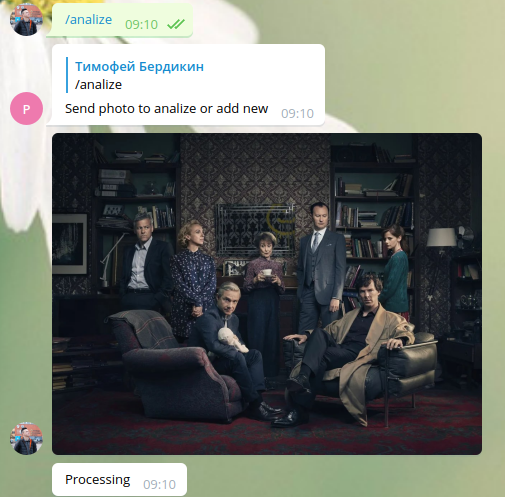
\includegraphics{picture2} \linebreak

\includegraphics[scale=0.5]{picture3} \linebreak
\section*{Ссылка на GitHub}

\pagebreak


\end{document}

